%  $Description: Thesis
%  $Author: xxx $
%  $Date: xxx  $
%  $Revision: 0.0 $

\documentclass[11pt]{book}
\usepackage{LNMIIT_BTP}
\usepackage{times}
\usepackage{epsfig}
\usepackage{amsmath}
\usepackage{amssymb}
\usepackage{latexsym}
\usepackage{url}
\usepackage{graphicx}
\usepackage{multirow}
\usepackage{algorithm2e}
\usepackage{graphicx}
\usepackage[english]{babel}
\usepackage{blindtext}
\graphicspath{{Figures/}{./}} % To include images in other directories
%\usepackage{setspace}

\long\def\symbolfootnote[#1]#2{\begingroup%
\def\thefootnote{\fnsymbol{footnote}}\footnote[#1]{#2}\endgroup}
\renewcommand{\baselinestretch}{1.2}
\onecolumn
%--------------------------------------------------------

\begin{document}
\pagenumbering{roman}

%%Cover Page
 

%% TITLE PAGE
 \thispagestyle{empty}
\begin{center}
{\Large \bf Security Of Modern Computing Environment(cloud and Fog computing)  }

\vspace*{1.75cm}
{\large Project report submitted in partial fulfillment\\}
{\large  of the requirements for the degree of \\}

\vspace*{1cm}
{\it {\large Bachelor of Technology} \\
{\large in\\}
{\large Computer Science Engineering  \\}}

\vspace*{1cm}
{\large by}

\vspace*{1cm}
{\large LOKESH KAUSHIK - 14UCS059\\}
{\large HARSH THAKUR - 14UCC011\\}
{\large SUDHANSHU SINGH - 14UCS128\\}
{\large  SIYARAM SAURABH DWIVEDI- 14UEC104\\}


\vspace*{5mm}
{\large Under Guidance of \\}
{\large Mr. Hemant Kumar Mehta \\}
{\large Associate Professor, Computer Science Engineering \\}

\vspace*{3.0cm}
{\psfig{figure= Figures/LNMIIT.png ,width=44mm}\\}
{\large Department of Computer Science Engineering \\}
{\large The LNM Institute of Information Technology, Jaipur\\}

\vspace*{1.0cm}
{\large May 2018\\}
\end{center}




%% CERTIFICATE PAGE
\newpage
\thispagestyle{empty}
\vspace*{1.5cm}
\begin{center}
{\Large The LNM Institute of Information Technology\\}
{\Large Jaipur, India\\}
\vspace*{3cm}
{\Large \bf CERTIFICATE\\}
\vspace*{1cm}
\noindent
\end{center}
    This is to certify that the project entitled “Security of Modern Computing Environment(cloud and Fog computing)” , submitted by Lokesh Kaushik (14ucs059), Harsh Thakur (14ucc011) and Sudhanshu Singh (14ucs128), Siyaram Saurabh Dwivedi(14uec104) in partial fulfillment of the requirement of  degree in Bachelor of Technology (B. Tech), is a bonafide record of work carried out by them at the Department of Computer Science Engineering, The LNM Institute of Information Technology, Jaipur, (Rajasthan) India, during the academic session 2017-2018 under my supervision and guidance and the same has not been submitted elsewhere for award of any other degree. In my/our opinion, this thesis is of standard required for the award of the degree of Bachelor of Technology (B. Tech).

\vspace*{3cm}
\begin{tabular}{cc}
\underline{\makebox[1in]{}} & \hspace*{5cm} \underline{\makebox[2.5in]{}} \\
Date & \hspace*{5cm} Adviser: Mr. Hemant Kumar Mehta
\end{tabular}
\oneandhalfspace


%\mastersthesis
%\renewcommand{\baselinestretch}{1.5}

% ACKNOWLEDGEMENTS PAGE
\chapter*{Acknowledgments}
\label{ch:ack}

This project of ours would not have been a success without the helping hands of our fellow friends and patient mentors. We would like to thank a few of them for their selfless work with us. First and foremost, we would like to express our gratitude towards our mentor and distinguished faculty Dr. Hemant Mehta  who had been a continuous support since the inception of the project. Also, we would like to thank our some friends and batchmates who always helped us whenever we were stuck anywhere. 


% Abstract
\chapter*{Abstract}
\label{ch:abst}
Cloud computing is associate degree rising paradigm for big scale infrastructures.It
has the advantage of decreasing expense by sharing process and capability assets, joined with associate degree on-request provisioning component reckoning on a compensation for each utilization arrange of action.But the chief concern in cloud environments is to supply security around multi-tenancy and isolation.Security at totally different levels such as Network level, Host level and Application level is critical to stay the overcloud and running continuously. 

The security downside becomes additional difficult beneath the cloud models as new
dimensions have entered into the matter scope associated with the model design,multi-tenancy, snap and layer dependency stack. we tend to introduce a close analysis of the cloud security downside. we tend to investigated the problem from the cloud design perspective.Also provided potential measures to urge prevented from
these attacks exploitation numerous security technique and within the last half we
tend to use NESSI2 package and showed the simulation for DDOS attack and generated its report, graphs and wrote conclusion.

Fog computing is an architecture which end-user clients or nearby edge devices to carry out a considerable amount of storage , communication
, control , measurement and management rather than controlled primarily by network gateways.In fog computing, for any instance of time same
edge device can be used by multiple smart applications with different set of users which raises the issue of security of edge device.Attacks in fog computing
can be classified into two main categories (a) unauthenticated attacks and (b) unauthorized attacks . Attack detection in fog computing is done by using 
machine learning algorithms , we use machine learning because it automatically improves with experince and enchance its capabilites .Attack detection could benefit from a
pre-training scheme of stacked autoencoders for automatic feature learning. One way to apply stacked
autoencoder is to train a model with a mix of normal/attack sample of the unlabeled network so that the
model identifies patterns of attack and normal data by a self-learning scheme. The detected patterns are
mapped to labeled test data as attack and normal.

Our work is to design and implement deep learning based mechanism this work has used self taught deep learning scheme in which unsupervised feature learning has
been employed on training data.The learnt features were applied to the labeled test dataset for classification into attack and normal .
We used NSL-KDD intrusion dataset which is available in csv format for model validation and
evaluations. The original dataset consists of 125,973 records of train and 22,544 records of test, each
with 41 features such as duration,protocol, service, flag, source bytes, destination bytes, etc.
We have used k-fold cross validation to check the accuracy of our model and generated its report and wrote conclusions. 




%--------------------------------------------------------
\tableofcontents
%\listoffigures
%\listoftables

%----------------------------------------------------
\chapter{A survey on cloud computing}
\section{Introduction}
In the initial years of the 60s,computers required giant rooms and consumed giant amounts of electricity, had dear electronic elements and made little or no process output.However,smaller computers eventually replaced those room-size computers.At the top of the last century,the magnitude of computing and infra- structure node organized to make a distributed system, that provided a rise in efficiency. In recent years,when the demand of information and on line users has immensely in- rumpled,the ancient computing infrastructure is turning into costlier and tougher to manage.Traditional computing is not suitable for accessing knowledge any wherever and at anytime.In order to try to to therefore, we'd like to save lots of the info on Associate in Nursing auxiliary storage system.Ad- ditionally, the rise of on-line users on networking sites, online surfing, video conferencing,and such can not be handled by ancient computing.
Distributed computing is one amongst the foremost blazing center specialised subjects within the advanced time. it's developed with expansive going impacts crosswise over IT, organizations, programming building and data stockpiling. one amongst the principle impacts is that the growth of their ability. This increase in capability does not essentially mean a rise in expenses in hardware, software, and coaching of private to mention many. in keeping with the National Institute of Standards and Technology (NIST) definition, the cloud computing could be a model for facultative convenient, resource pooling, ubiquitous, on-demand access which can be simply delivered with differing types of service supplier interaction. The cloud computing follows easy pay as you go (PAYG) model, wherever you get the services youve used. One of the main edges of PAYG model is that we are able to cut back our expenditure by provisioning a particular amount of resources. The user will choose processor, memory, hard disk, software package, networking, access management and any extra new package PRN to their setting. The resources provided on-demand to the client or finish users. It provides tremendous edges to business and residential users and attracts the eye of the analysis community Cloud computing implements virtualization technique is to produce resources with efficiency to the tip user. The characteristics of cloud computing include tractableness, quantifiability, and handiness. additionally, cloud computing is additionally economical, on-demand service, expedient, ubiquitous, multitenant, elasticity, and stability. Cloud computing offers mainly 3 service delivery models; Infrastructure as a Service (IaaS), Platform as a Services (PaaS)
and software system as a Service (SaaS). office defines four-development model of the cloud: public, private, hybrid and community. Cloud computing uses cloud server stack wherever the shopper or user is on the front end and server on the rear finish. Services reside in middleware of stack as shown in Fig. 1. At the top level resides the appliance, that directly delivers the outsourced software system to the shopper and eliminates sophisticated software system. Customers do no got to expend cash to put in software system, solely they obtain their usage.\begin{figure}
	\centering
	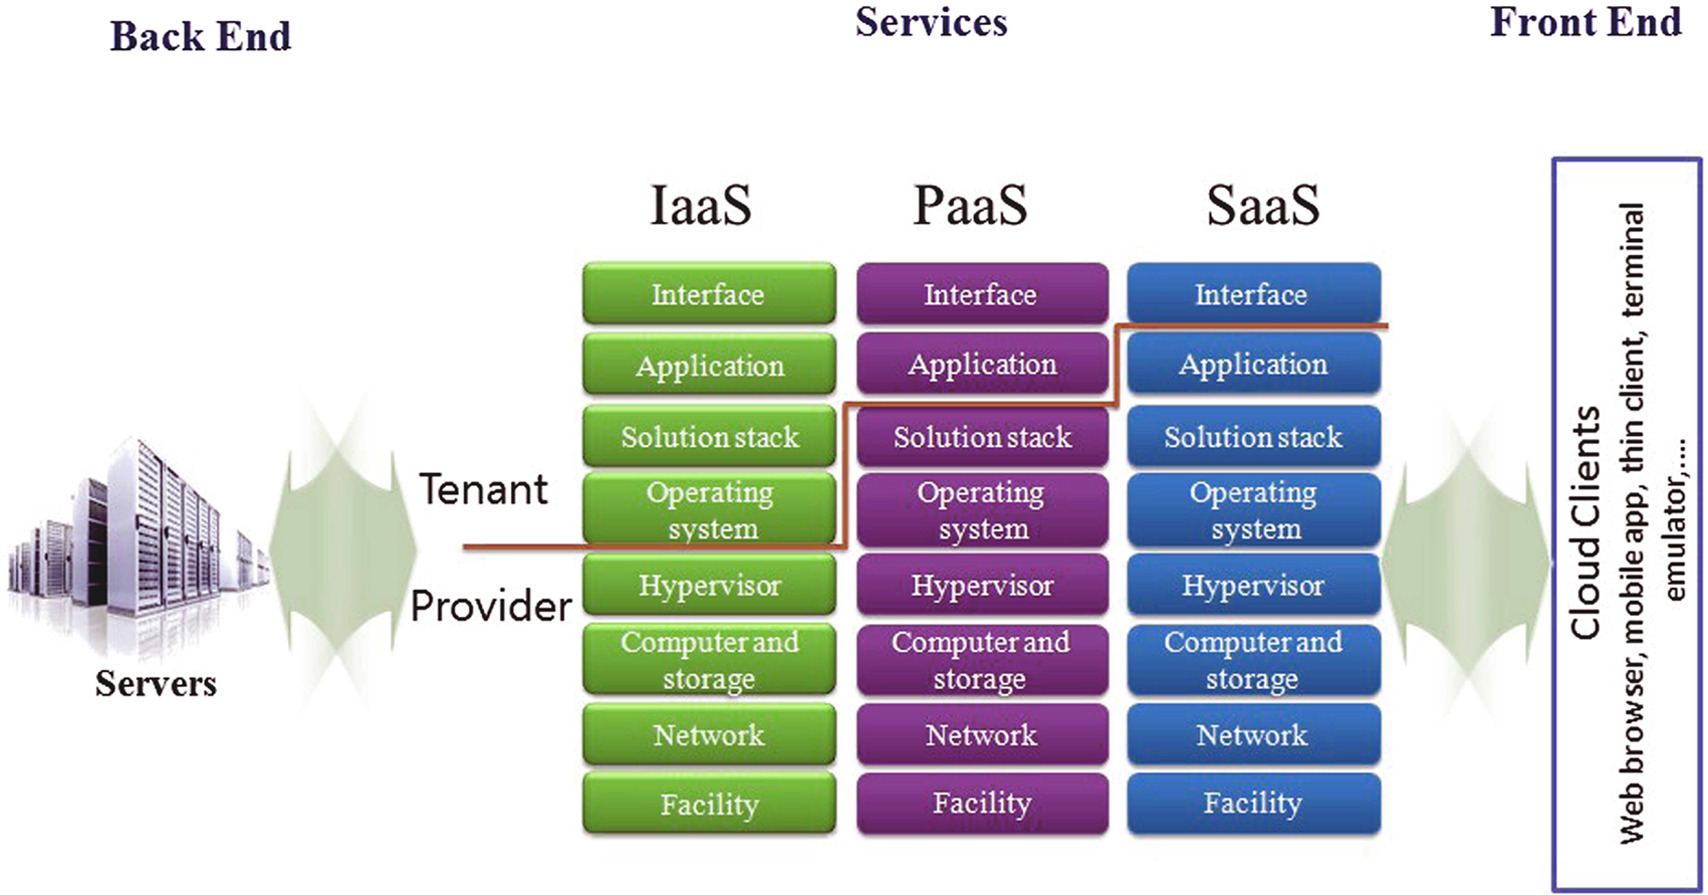
\includegraphics[width=\linewidth]{cloud.jpg} 
	\caption{Cloud service delivery models}
	\label{fig:cloud}
\end{figure}


NIST is accountable for developing tips and standards to produce security in cloud atmosphere.Here we have a tendency to outline the cloud design as a fourfold, that consists of: (a) cloud computing concept and characteristics (b) cloud deployed models (c) cloud service delivery models (d) cloud security concept. the small print of the cloud design ar given below:

\section{Cloud service delivery models}
the major 3 delivery models ar IaaS, PaaS, and SaaS. Still several service models ar accessible as per their practicality and repair providing capabilities, that have LED to the creation of Anything as service AaaS delivery models. during this section, we have a tendency to discuss the various styles of service models as shown

\textit{Infrastructure as a service (IaaS)} It belongs to all-time low of the model. IaaS deals with pc hardware (network storage, virtual server/machine, knowledge center, processor, and memory) as a service. IaaS supports the revolution within the business investment in IT infrastructure The snap of allocating physical or virtual resources helps providing the infrastructure in associate degree abstract manner. It additionally provides scalability and provisions (such as hypervisor) problems with infrastructure while not the requirement of paying huge quantity of funds and time.


\textit{Platform as a service (PaaS):} it is in middleware of service model and it delivers the services in the form of development tools, framework, design, programs, and Integrated Development Environments(IDE). In alternative words, the purchasers area unit ready to management the
applications however do not have any means to manage the underlying infrastructure. It will be useful in things wherever multiple developers located in several physical locations ought to work along. a well-liked PaaS supplier is Google App
Engine. it's a software package Development Kit (SDK) that provides associate
degree atmosphere that supports Python, Java, and Go programming languages. because it provides options that area unit prepared for the client, PaaS is more extensile and additional versatile than SaaS model.

\textit{Software as a service (SaaS)}  (SaaS) it is a set of remote computing services. SaaS is at the highest model among the delivery models. It permits the applications to deploy remotely by third-party vendors. It allows the client to use cloud service provider’s application (CSP’s) running on cloud infrastructure
via the web. SaaS is that the prevailing cloud market and still keeps growing quickly. Google App and Salesforce area unit samples of SaaS suppliers.

\begin{figure}[h]
	\centering
	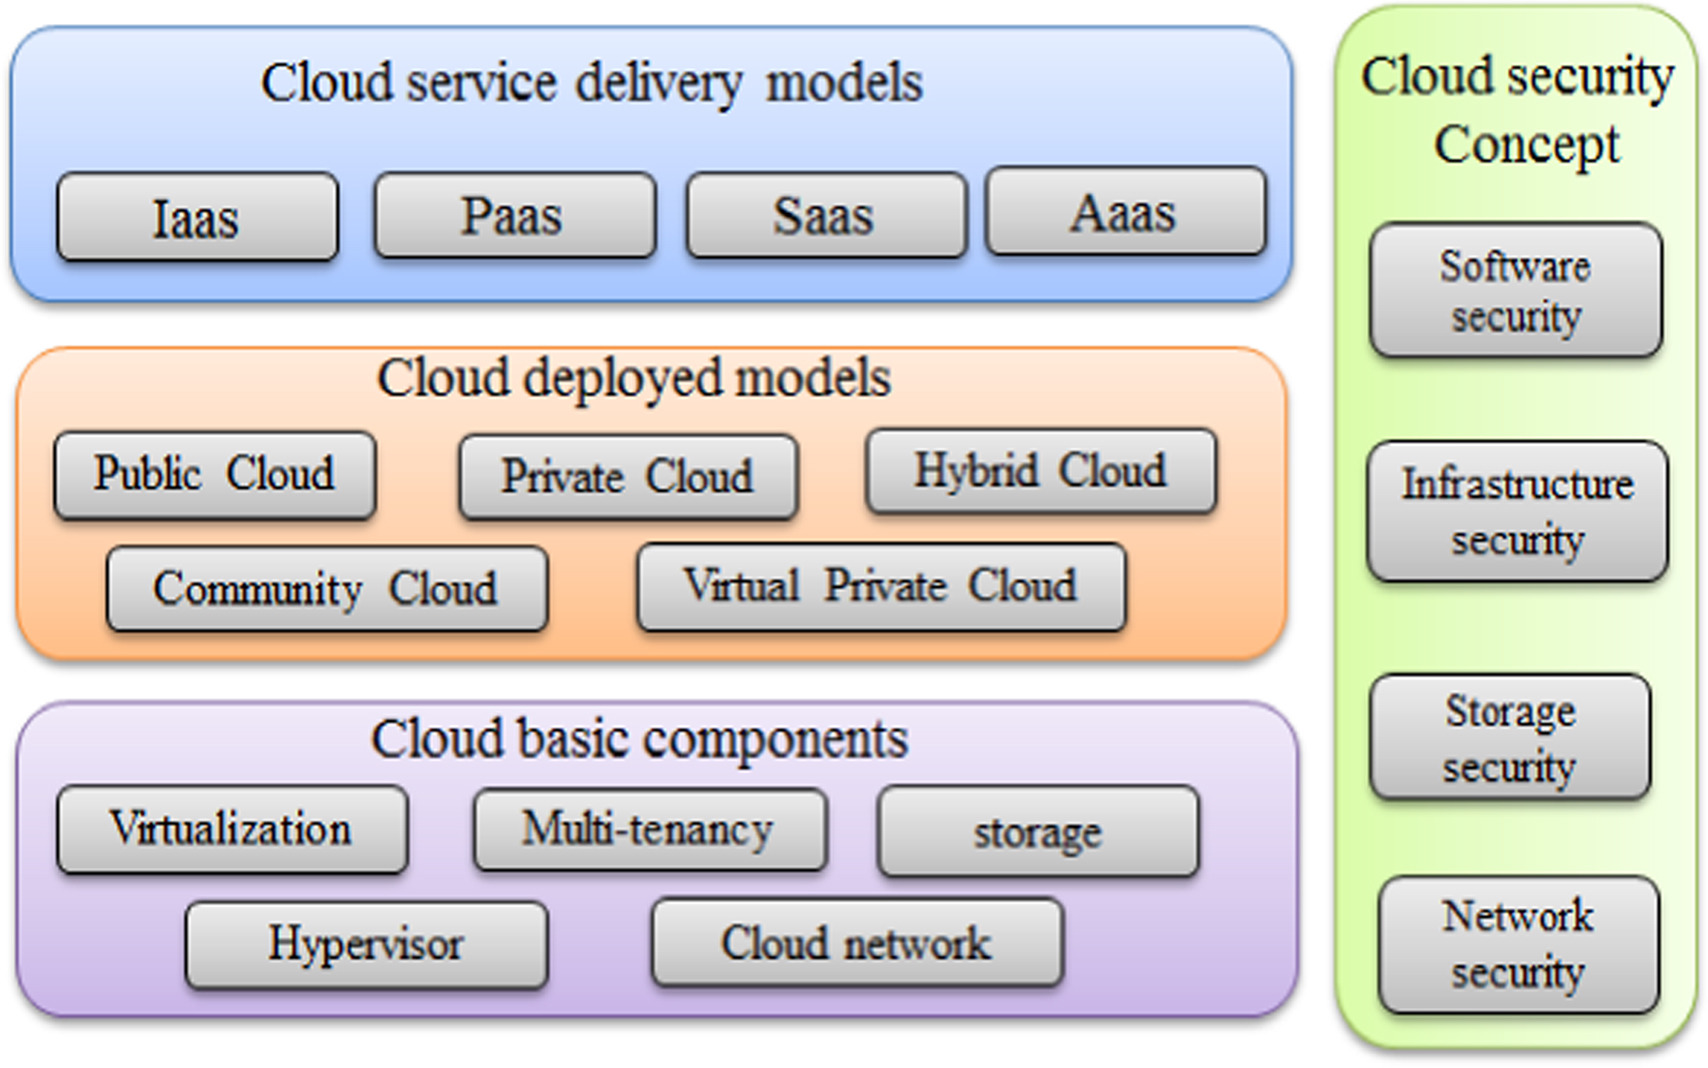
\includegraphics[width=\linewidth]{ServiceModels.JPG}
	\caption{Cloud computing framework}
	\label{fig:service-models}
\end{figure}


\textit{Anything as a service (AaaS)} it is a collective term which mixes variety of things as X as a service. X is also something or everything as a service. This service becomes interchangeable in cloud landscape. The cloud system area unit ready to support the massive resource to specific, personal and granular necessities mistreatment Monitor as a Services (MaaS), knowledge as a
Service (DaaS), Communication as a Service (CaaS), Security as a Service (SecaaS), Routing as a Service (RaaS).


\section{Cloud deployed models}
Cloud computing typically depends on shared resources by native servers or individual devices. Therefore, it is able to come through consistency by taking the advantage of resource sharing. Deployed model tells what is the aim and nature of the cloud. By doing this, it reduces the facility of servers, capital expenditure and management the disbursal. bureau defines 5 styles of deployed models:

•\textit{ Private cloud}: Cloud computing operates and manages inside the info center of a corporation is called a personal cloud. several shoppers of cloud infrastructure (eg, business units) are together with provision for exclusive use by one organization. in an exceedingly personal cloud, it is abundant easier to spot the customer and merchant relationship as a result of the infrastructure in hand and operated by constant organization. Therefore, security risks area unit easier to notice.

•\textit{Public cloud:} it is truth illustration of cloud hosting wherever the client and supplier have a strong Service Level Agreement (SLA) to take care of the trust between them. during this cloud infrastructure, open access to the general public and organization provided. Businesses, academics, or governmental organizations own public cloud environments. this suggests multiple entities could own and operate a public cloud. This creates several problems, as we tend to dont recognize wherever the resources area unit settled or World Health Organization owns them, increasing the issue of protective them from attack.

\textit{Community cloud:} Cloud infrastructure of the organizations shared considerations(mission, security necessities,policy, and compliance considerations) of shoppers a special provision has been created for exclusive use by the community model. it is in hand, managed, and community organizations, a third party, or some combination of them is driven by one or additional, which could also be gift on or off field. In easy words, a community cloud is being shared and controlled by multiple organizations.

\textit{Hybrid cloud:} it is the mix of 2 or additional clouds (public, private, community). Usually, the data and application area unit sure along by standardized and behaviour technology. Hybrid cloud offers the advantages of various clouds readying models. However, it is well organized and safer than public cloud whereas accessing the entities over the net.

\textit{Virtual private cloud:} It is a semi-private cloud, which is fewer resources, and it consists of virtual private network (VPN). It is on demand configurable pool of shared resources allocated within the cloud environment.

\section{Cloud computing basic component}
 
 In this section, we will discuss the fundamental parts on that cloud computing deployed. These components incorporates a large vary of services that we are able to use everywhere the net. Here we have a tendency to discuss some vital component:
 
 \textit{ Virtualization:} It plays a vital role in deploying the cloud. it is the strategic part in the cloud, that permits the physical resources by multiple shoppers. It creates the virtual instance of resource or device like software system, servers, network resources and storage devices whereby the framework utilize the resources into quite one execution surroundings.
 
 \textit{ Multi-tenancy:} Multi-tenant surroundings will have multiple customers or users who doesn't see or share every other’s knowledge however will share resource or application in Associate in Nursing execution surroundings, although they
 may not belong to identical organization. Multi-tenancy results the optimum utilization of hardware and data storage mechanism.
 
 \textit{Cloud storage:} It is a component, which maintained, managed, and backed up remotely and it made available over the network where the users can access data.

 \textit{The hypervisor:} The thus referred to as virtual machine monitor or manager could be a key module of virtualization. It permits multiple Virtual Machines (VMs) to run on one hardware host. It manages and monitors the various in operation systems, that run in a very shared physical system.
 
 \textit{Cloud Network:} It will operate quite one standard knowledge centers, a typical knowledge center contains hundreds or thousands of servers. To expeditiously build and manage the storages the cloud needs a secure network infrastructure referred to as cloud networking. It needs an online affiliation and similar with a virtual personal network that permits the user to firmly access printers, applications, files etc.








\chapter{Threats To Security In Cloud Computing}
\label{ch:Threats}
\section{Introduction}
The main worry in cloud conditions is to present security around multi-occupancy and
disengagement, giving shoppers additional solace aside from believe United States thought of mists. There has been review works elaborated that orders security dangers in cloud in lightweight of the concept of the administration conveyance models of a distributed computing framework. Not with standing, security needs Associate in Nursing all encompassing methodology. Service delivery model is one in all several aspects that require to be thought of for a comprehensive survey on cloud security. Security at completely different levels like Network level, Host level and Application level is critical to stay the cloud over and running ceaselessly. As per these distinctive levels, different forms of security breaks might happen. These are organized in remainder of
this phase. 
\section{Basic Security}
Web 2.0, a key technology towards enabling the employment of computer code as a
Service (SaaS) relieves the users from tasks like maintenance and installation of computer code. it's been used wide all around. As the user community victimization internet a pair of web 2.0 is increasing by leaps and bounds, the protection has become a lot of important than ever for such atmosphere.

\textit{SQL injection attacks}: These attacks ar the one within which a malicious code is inserted into a customary SQL code and so the attackers gain unauthorized access to a information and become able to access sensitive info. typically the hackers input file is misunderstood by the web-site because the user data and permits it to be accessed by the SQL server and this lets the wrongdoer to
own power of the functioning of the web site and build changes into that. numerous techniques like: avoiding the usage of dynamically generated SQL within the code, victimization filtering techniques to sanitize the user input etc to ascertain
the SQL injection attacks.

\textit{Cross Site Scripting (XSS) attacks} :that inject malicious scripts into internet contents became quite standard since the origination of internet a pair of web 2.0. supported the kind of services provided, an internet site is
classified as static or dynamic. Static sites dont expertise the sick effects of the
protection dangers that the dynamic sites do owing to their dynamism in giving multi-overlap administrations to the shoppers.

Another category of threat alright best-known to SaaS ar named as Man within the
Middle assaults. In such an assault, a intruder tries to interpose in an exceedingly progressing discussion between a sender and a client to infuse false information and to grasp regarding the imperative info changed between them. Different devices capital punishment solid coding advances like Dsniff, Cain, Ettercap, Wsniff, Airjack so on have been made keeping in mind the top goal to offer defend against them.
\section{Network Level Security}
 To ensure network security following points like confidentiality and integrity within the network, proper access management and maintaining security against the external third party threats ought to be thought-about while providing network level security. issues related to the network level security comprise of: DNS attacks, individual attacks, issue of reused informatics address,Denial of Service (DoS) and Distributed Denial of Service attacks (DDoS) etc.

\textit{DNS ATTACKS :}
A domain Name Server (DNS) server performs the interpretation of a website name
to associate informatics address. Since the domain names area unit a lot of easier to recollect. Hence, the DNS servers are needed. however there area unit cases once having referred to as the server by name, the user has been routed to
some other evil cloud rather than the one he asked for and thus victimization
informatics address isn't continually possible.
Although victimization DNS security measures like: name System Security
Extensions(DNSSEC) reduces the results of DNS threats however still there area unit cases once these security measures encourage be inadequate once the trail between a sender and a receiver gets rerouted through some evil association.

\textit{SNIFFER ATTACKS :}
These varieties of attacks area unit launched by applications which will capture packets flowing in a very network and if the info that is being transferred through these packets don't seem to be encoded, it can be perused and there area unit probabilities that key knowledge streaming over the system are often followed or caught. A sniffer program, through the NIC (Network Interface Card) guarantees that the information/movement connected to completely different frameworks on the system likewise gets recorded. It are often achieved by putting the NIC in promiscuous mode and in promiscuous mode it will track all knowledge, flowing on a similar
network. A malicious sniffing detection platform supported Arp (address resolution
protocol) and RTT (round trip time) are often wont to find a sniffing system running on a network.

\textit{ISSUE OF REUSED IP ADDRESSES :} every node of a network is provided
associate informatics address and thus an informatics address is largely a finite amount. an outsized variety of cases associated with re-used IP-address issue
have been discovered of late. At the purpose once a selected consumer moves out
of a system then the IP-address related with him (before) is dealt out to a different consumer. This sometimes probabilities the protection of the
new consumer as there is a certain time slack between the distinction in associate
informatics address in DNS and also the clearing of that address in DNS stores. what's additional, thus, we are able to state that sometimes but the previous informatics deliver is being dealt out to a different consumer still the chances of aiming to the knowledge by another client isn't immaterial because the address still exists within the DNS store and also the data having an area with a selected consumer could find yourself perceptibly obtainable to another consumer damaging the protection of the first consumer.
\section{Application Level Security}
Application level security refers to the usage of software system and hardware
resources to produce security to applications such the attackers don't seem to be ready to get management over these applications and create desirable changes to their format.Now a days, attacks ar launched, being disguised as a trustworthy user
and the system considering them as a trustworthy user,allow full access to the
assaultive party and gets victimized. the explanation behind this can be that the superannuated network level security policies permit solely the authorized users to access the precise informatics address.

\textit{SECURITY CONCERNS WITH THE HYPERVISOR :}
Cloud Computing rests primarily on the idea of virtualization. in a very virtualized world, hypervisor is outlined as a controller popularly called virtual
machine manager (VMM) that enables multiple operational systems to be run on a
system at a time, providing the resources to every software such they are doing not interfere with each. because the amount of working frameworks running on Associate in Nursing instrumentation unit increment, the safety problems distressed concerning thos that of latest operating frameworks likewise ought to be thought of. Since varied operating frameworks would keep running on a solitary instrumentation stage, it's not conceivable to watch all and after
keeping up all the operating frameworks secure is hard. it would happen that a visitant framework tries to run a pernicious code on the host framework and cut the framework down or take full management of the framework and piece access to alternative visitant operating frameworks.

\textit{DENIAL OF SERVICE ATTACKS :}
A DoS attack is a trial to create the services appointed to the licensed users unable to be employed by them. In such Associate in Nursing attack, the server providing the service is flooded by an oversized variety of requests and thence the service becomes unprocurable to the licensed user.
Sometimes, we tend to attempt to access a website we see that as a
result of overloading of the server with the requests to access the positioning, we tend to ar unable to access the positioning and observe miscalculation. This happens once the amount of requests that may be handled by a server exceeds its capability. The prevalence of a DoS attack will increase bandwidth consumption besides inflicting congestion, guaranteeing components of the clouds inaccessible to
the users.

\textit{COOKIE POISONING :}
It involves dynamic or modifying the contents of cookie to create unauthorized
access to Associate in Nursing application or to a webpage.Cookies essentially
contain the users identity connected credentials and once these cookies ar accessible, the content of those cookies may be solid to impersonate an authorized user. this could be avoided either by playacting regular cookie cleanup or implementing an coding theme for the cookie information.

\textit{BACKDOOR AND DEBUG OPTIONS :} a typical habit of the developers is to change
the right option whereas publication a web-site. this permits them to create biological process changes within the code and get them enforced within the web-site. Since these right choices facilitate backend entry to the developers, and typically these right choices ar left enabled unremarked, this could give a simple
entry to a hacker into the web-site and let him create changes at the web-site level.

\textit{DISTRIBUTED DENIAL OF SERVICE ATTACKS :} DDoS is also referred to as a
complicated version of DOS in terms of denying the vital services running on a server by flooding the destination sever with Associate in Nursing many variety of packets such the target server isn't ready to handle it. In DDoS the attack is transferred from varied dynamic systems that have simply been listed off dissimilar to DOS. The aggressors have the flexibility to manage the stream information by allowing some data accessible at bound times.Thus the add and type of knowledge accessible for open utilization is plainly underneath the management of the
assailant.The DDoS attack is pass 3 purposeful units: A Master, A Slave and A Victim. Master being the attack launcher is behind of these attacks inflicting DDoS, Slave is that the network that acts like a launch pad for the Master. It provides the platform to the Master to launch the attack on the Victim.
Hence it's conjointly known as as co-ordinated attack.

\textit{CAPTCHA BREAKING :}
CAPTCHAs were developed so as to stop the usage of web resources by bots or computers. they are accustomed stop spam and development of network resources
by bots. Even the multiple web-site registrations, lexicon attacks etc by an automatic program ar prevented employing a CAPTCHA. however recently, it's been found that the spammers ar ready to break the CAPTCHA, provided by the Hotmail and G-mail service suppliers. they create use of the electronic equipment able to scan the CAPTCHA characters for the visually impaired users and use speech to text conversion software to defeat the check.

\textit{GOOGLE HACKING :}
Google hacking refers to mistreatment Google computer programme to search out sensitive info that a hacker will use to his profit whereas hacking a users account. Generally, hackers try and realize out the safety loopholes by inquiring out on Google regarding the system they want to hack and so when having gathered the mandatory info, they perform the hacking of the involved system.
In some cases, a hacker isn't positive of the target. Instead he tries to Google out the target supported the loophole he wishes to hack a system upon. The hacker then searches all the attainable systems with such a loophole and finds out those having the loopholes he desires to hack upon. A Google hacking event was ascertained
recently once login details of assorted g-mail users were purloined by a gaggle of
hackers in China. These had been a number of the safety threats that may be launched at the applying level and cause a system downtime disabling the applying access even to the licensed users.






\chapter{Ensuring Security Against The Various Types Of Attacks}
\label{ch:Mitigations}
\section{Introduction}
In order to secure the cloud against the varied security threats and attacks like: SQL injection, Cross Site Scripting (XSS) attacks, DoS and DDoS attacks, Google Hacking and compelled Hacking, different cloud service suppliers adopt completely different techniques. a number of normal techniques so as to observe the above mentioned attacks area unit as: Avoiding the usage of dynamically generated
SQL within the code, finding the meta-structures employed in the code, confirmative all user entered parameters, disallowing and removal of unwanted knowledge and characters, etc. A generic security framework must be found out for AN optimized value performance magnitude relation. the most criterion to be stuffed up by the generic security framework are to interface with any style of cloud atmosphere, and to be ready to handle and observe predefined as well as bespoke security policies. an identical approach is getting used by Symantec Message LabsWeb Security cloud that blocks the protection threats originating from web and filters the info
before they reach the network. net security clouds security design rests on 2 components:
\textbf{a. Multi layer security:} so as to confirm that knowledge security and block potential malwares, it consists of multi-layer security and therefore a robust security platform.
\textbf{b. URL address filtering:} it's being determined that the attacks area unit launched through numerous web content and websites and therefore filtering of the web-pages, ensures that no such harmful or threat carrying web page gets accessible. Also, content from undesirable sites will be blocked. With its
elastic technology, it provides security even in extremely conflicting environments and ensures protection against new and convergency malware threats.
\section{Man In Middle attacks :}
If secure socket layer (SSL) is not properly configured, then any attacker is able to access the data exchange between two parties. In Cloud, an attacker is able to access the data communication among data centers.

\textbf{Mitigation:} Legitimate SSL setup and information correspondence tests between approved gatherings can be valuable to lessen the danger of Man-in- the-Middle assault.
\section{DoS and DDoS attacks : }
The symptoms to a DoS or DDoS attack are: system speed gets reduced and programs run very slowly, large number of connection requests from a large number of users, less number of available resources. Although when launched in full strength DDoS attacks are very harmful as they exhaust all the network resources. 

\textbf{Mitigation:} A careful monitoring of the network can help in keeping these attacks in control. 
\section{IP spoofing attacks: }
In case of IP spoofing an attacker tries to spoof the users that the packets are coming from reliable sources. Thus the attacker takes control over the client’s data or system showing himself as the trusted party.

\textbf{Mitigation:} Spoofing attacks can be checked by using encryption techniques and performing user authentication based on Key exchange. Techniques like IPSec do help in mitigating the risks of spoofing. By enabling encryption sessions and performing filtering at the incoming and outgoing entrances spoofing attacks can be reduced.
\section{Hypervisor attacks: }
VM-based rootkits initiate a hypervisor compromising the existing host OS to a VM.
The new guest OS assumes that it is running as the host OS with the corresponding control over the resources,however, in reality this host does not exist. Hypervisor
also creates a covert channel to execute unauthorized code into the system. This allows an attacker to control over any VM running on the host machine and to manipulate
the activities on the system.

\textbf{Mitigation:} The threat arising due to VM-Level
vulnerabilities can be mitigated by monitoring through
IDS (Instruction Detection System)/IPS (Intrusion
Prevention System) and by implementing firewall.

\chapter{Simulation Of DDOS attack Using Nessi2}
\label{ch:result}
\section{Features Of Nessi2}
NeSSi2 is designed to extend conventional network simulation tool features by supporting
detailed examination and testing opportunities of security-related network algorithms,
detection units and frameworks. The main focus of NeSSi2 is to provide a
realistic packet-level simulation environment as a testbed for the development of new
detection units as well as existing ones.NeSSi2 has been designed as a modular application with the focus on extensibility. In particular, NeSSi2 provides out-of-the-box support for various protocols of the TCP/IP stack.
\subsection{Traffic Generation}
Network traffic in the form of IP packets, complete with header and body, can be generated by different means. Implementing the TCP/IP protocol stack, NeSSi2 features an application layer module which is based on standard Java socket implementations.

NeSSi2 incorporates several application level protocols (HTTP, SMTP, etc.) and supports
static and dynamic routing protocols which can be selected by the user. At the
moment, static and dynamic protocols are implemented. A static routing protocol centrally computes the shortest paths as the network is loaded and each time the topology changes. The subsequent directing tables are thusly stacked onto the
individual system hubs. Then again, IS-IS(Intermediate- System-to- Intermediate-System) has been
actualized as a connection state convention, which depends on a decentralized calculation amid which
switches trade data about their connection states and assemble topology data locally.
\subsection{Protocol Stack and Socket-based API}
The routers as well as the end devices in the simulation contain a Network Layer; end devices also exclusively have a Transport and an Application Layer. At the Network Layer, IPv4 is realized with the key features global addressing, routing and fragmentation support. Moreover, TCP/IP model implementation allows containing several protocols in each layer; hence, Nessi2 also provide IPv6 support in NeSSi2. For the fault management, TTL (Time to live) and header checksums supported and the ICMP protocol has been implemented for failure notification.

Transport Layer is comprised of UDP and TCP. TCP in NeSSi2 offers a reliable and in-order delivery of data. Sockets represent the interface to the Application Layer, i.e., applications can set up several stream sockets as well as the corresponding server sockets. In this mold, outsider Java libraries can undoubtedly be incorporated in the recreation by substituting Java attachments with NeSSi2 attachments. All applications that are keep running in NeSSi2 take after a typical interface that edited compositions from their particular conduct however permits an institutionalized method for executing them. Right now, the HTTP, SMTP and IRC conventions are incorporated in NeSSi.
\subsection{Security Features}
The simulation setup in NeSSi2 is not only comprised of network creation and attachment
of traffic profiles, but additionally security related settings can be configured.
When a security framework composed of several detection units is to be tested, profiles
can also be used in NeSSi2 to simulate attacker behavior and attack patterns. NeSSi2 provides out-of-the box support for various attack scenarios such as bot networks initiating DDoS attacks. Here, infected end device nodes, “zombies”, are controlled by the bot net commander via the Internet Relay Chat application. The commander is capable of initiating different kinds of DDoS attacks like the SYN Flooding or UDP Storm. To this end, the attacker connects to an IRC communication server and sends attack commands to a chat channel all the bots are listening to. Therefore, the bots execute the coveted assault.
\section{Nessi2 Advantages}
\textbf{1) Scalability} - The user can use JAVA language to write application, and use Maven to define and adds the dependencies of the application. Therefore, Nessi2 can add functionality or application needed.

\textbf{2) Fidelity} - Nessi2 creates a network topology based on network characteristics, it also can automatically generate a network topology depended on the download file, it has high fidelity. (It can download the AS topology file from CAIDA website, then import into Nessi2, automatically generated network topology).

\textbf{3) Extensibility} - Nessi2 can work with third-party software, such as Wireshark.
\section{Components Of Nessi2}
\subsection{Graphical User Interface}

GUI of NeSSi2 has two use cases: On the one hand, results of running or terminated simulations can be visualized in here. On the other hand,
it is the component that allows the creation and modification of network topologies and scenarios.
A project consists of a root folder, some predefined sub folders and some files created by the user. The root folder is named after the project, whereas the sub folders are named after the element types they contain. NeSSi2 project files include the following types: networks, applications, profiles, scenarios, simulations, recorder configurations and the optional templates.
\begin{figure}[h]
	\centering
	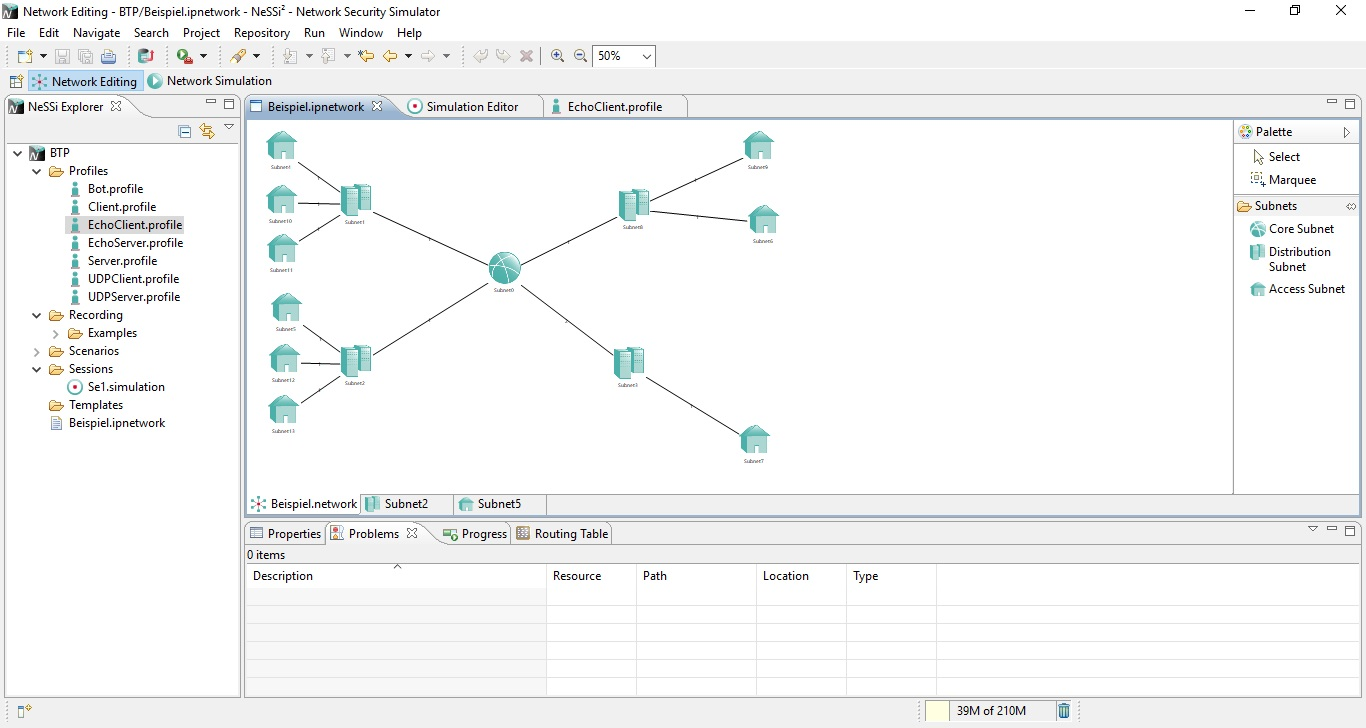
\includegraphics[width=\linewidth]{Nessi2GUI.JPG}
	\caption{GUI Of Nessi2}
	\label{fig:netwok}
\end{figure}

\newpage
\subsection{Simulation Backend}
The genuine reenactment is performed on a machine with equipment committed exclusively to this reason, the recreation backend.Once a reproduction is submitted for execution, the reproduction backend parses the coveted reproduction parameters (which occasion composes to log, what number of rushes to execute and so on.), makes a relating reproduction condition, sets up the database association and calendars the reproduction to keep running when the essential handling assets are accessible.NeSSi2 is built upon the JIAC framework, JIAC is a service-centric java-based middleware architecture based on the agent paradigm. Within NeSSi, agents are used for modeling and implementing the network entities such as routers, clients, and servers. The fundamental JIAC operator system gives a rich and adaptable reason
for actualizing and testing of different security arrangements and calculations in NeSSi2. Besides, expanding upon a specialist system permits joining the fractional information of the operators living in the system in a helpful approach for recognizing and in the end killing IP-based dangers.
\begin{figure}[h]
	\centering
		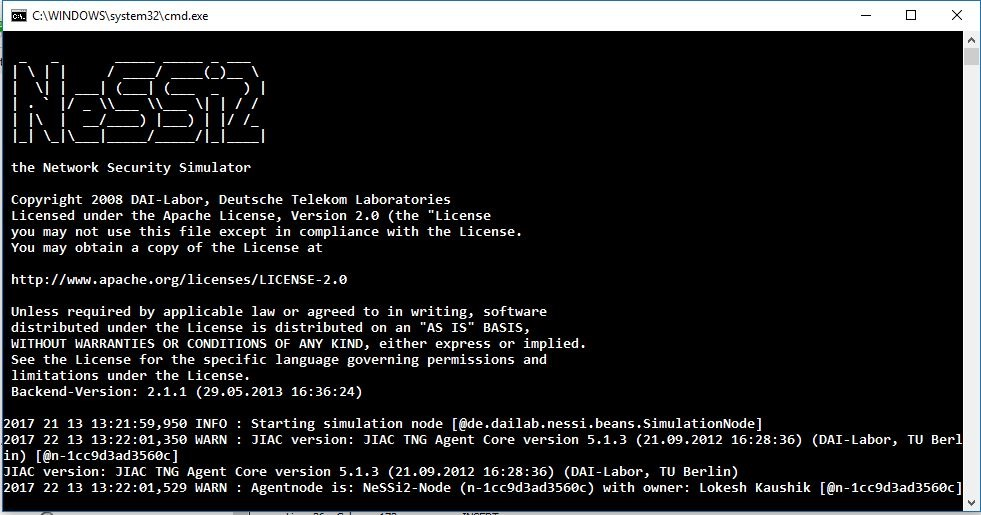
\includegraphics[width=\linewidth]{Backend.JPG}
	\caption{Nessi2 Backend}
	\label{fig:backend}
\end{figure}
\newpage
\subsection{Database}
The exact propagation of a reenactment empowers clients to utilize diverse discovery techniques or different arrangements of location units for a similar activity informational index. This permits the examination of execution and identification proficiency of various security system setups.For these purposes, we use a distributed database in which the traffic generated during a simulation is stored. For each simulation, the agents log the traffic and detection data and send it to the database that occurs in a simulated scenario between a start and end time. The data types to be logged are specified by the user in the simulation parameters.The network model is saved in an XML file.
\newline
Due to the modular design of the database component, the actual implementation of the
database is up to the user. This can be comfortably managed via the graphical user interface, where the location of the database, database user name, password and the database driver can be specified. NeSSi2 has been tested extensively with a MySQL database server, but depending on the user’s preferences, this can easily be substituted by another module.

\section{How we created DDOS simulation}
\subsection{Create Nessi2 Project}
As a first step a NeSSi2 project has to be created using the NeSSi2 project creation
wizard. This wizard can be accessed in two ways in the NeSSi2 GUI. One way is by
the following menu sequence: File-> New-> IP Network(Project).

\begin{figure}[h]
	\centering
	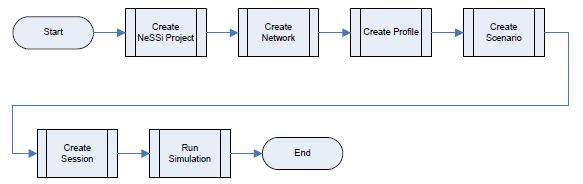
\includegraphics[width=\linewidth]{procedureJPG.JPG}
	\caption{}
	\label{fig:procedure}
\end{figure}
\subsection{create Network}
The nodes and edges of each network are grouped in subnets. Hence, the first step of creating a network is defining some subnets for the network. The available subnet types are listed in the palette located on the right side of the Network Editor Via drag and drop we can add the subnets to the network.
The next step after adding subnets to the network is to add content to the subnets. In
order to do so, double click on a subnet. This will cause for a new tab to be opened
in the Network Editor. Same as with the subnets, the palette will display a list of the
available nodes and edges. By dragging and dropping nodes, they will be added to the
network. For connecting nodes, we will have to select one of the links found in the
Connections part of the palette and than clicking on the nodes that we want to connect.
We also have to connect the subnets to each other. In this case, we  have to select an network element (usually the routers) and enter its context menu. Select Connect to Subnet, then select the subnet we  want to connect to. This will cause for the network device to appear in both subnets.
\begin{figure}
	\centering
	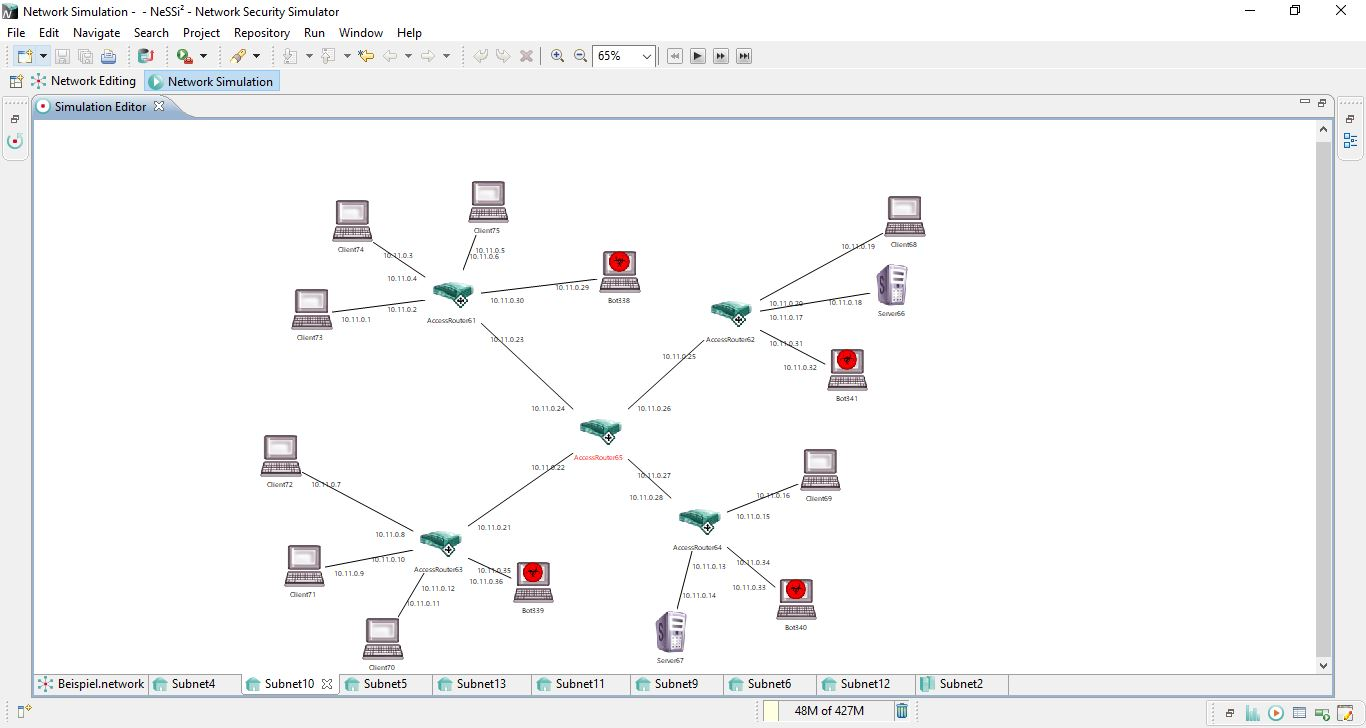
\includegraphics[width=\linewidth]{subnet.JPG}
	\caption{Network design of subnet}
	\label{fig:subnet}
\end{figure}

\newpage
\subsection{Create Profile}
A profile is basically a container for a set of applications.Explorer and selecting New->Profile.This will open a dialog where a name has to be entered for the profile. By pressing "Finish", the dialog will close and a file with the .profile extension will be created in the Profiles folder of the project. Now, applications may be added to the profile.By pressing the Add... button in the newly created profile, we can add applications to the profile.
\subsection{Create Scenario}
A scenario is the mapping of profiles onto the nodes of a specific network.A scenario defines which profiles are deployed on each node of the network topology.
Multiple profiles may be deployed on the same node simultaneously. Analogous to the
profiles, the scenarios are stores in the Scenarios directory of each project with .scenario file extension and XML-based content.
\subsection{Create Simulation}
As the core element of simulation execution, simulations are the components that can be
launched from within the user interface and evaluated in the backend. Simulation files
have .simulation file extension and XML-based content and are located in Sessions
folder of a project.The duration of a simulation execution is determined by two parameters, namely replications and ticks. Replications specify how many times a scenario is to be executed, whereas ticks are the time units by which runs are measured.
\subsection{Recorder Configurations}
Recorder configurations specify the event types that are to be recorded during the simulation execution in NeSSi2 Backend onto the database. The default configurations can
be found in Recordings/Examples folder of each NeSSi2 project.
\newpage
\section{Results and simulation}
\begin{figure}[h]
	\centering
		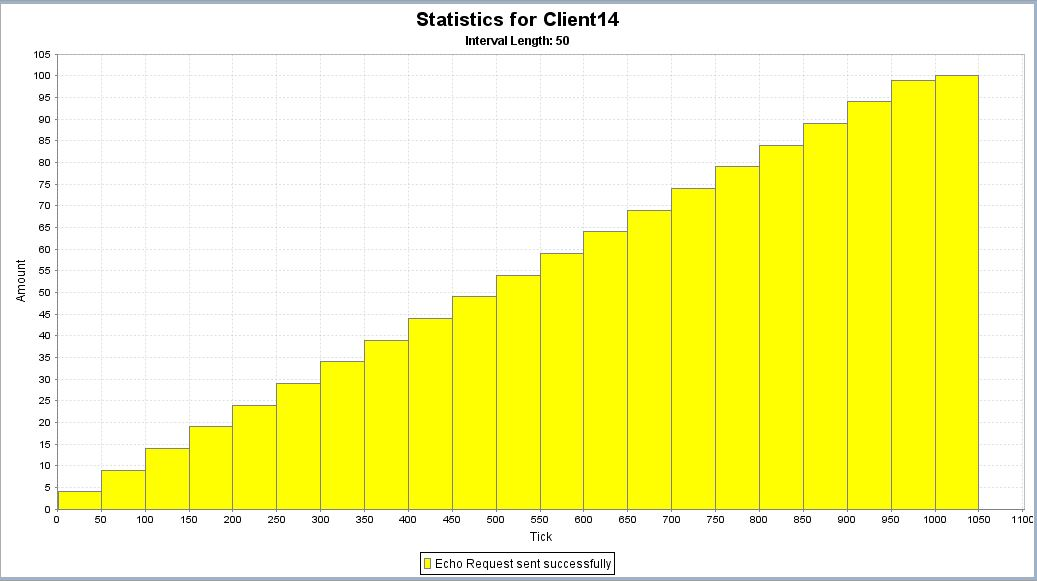
\includegraphics[width=\linewidth]{Client14.JPG}
	\caption{}
	\label{fig:client10}
\end{figure}
\begin{figure}[h]
	\centering
		\includegraphics[width=\linewidth]{Client74.JPG}
	\caption{}
	\label{fig:client13}
\end{figure}
\begin{figure}[h]
	\centering
		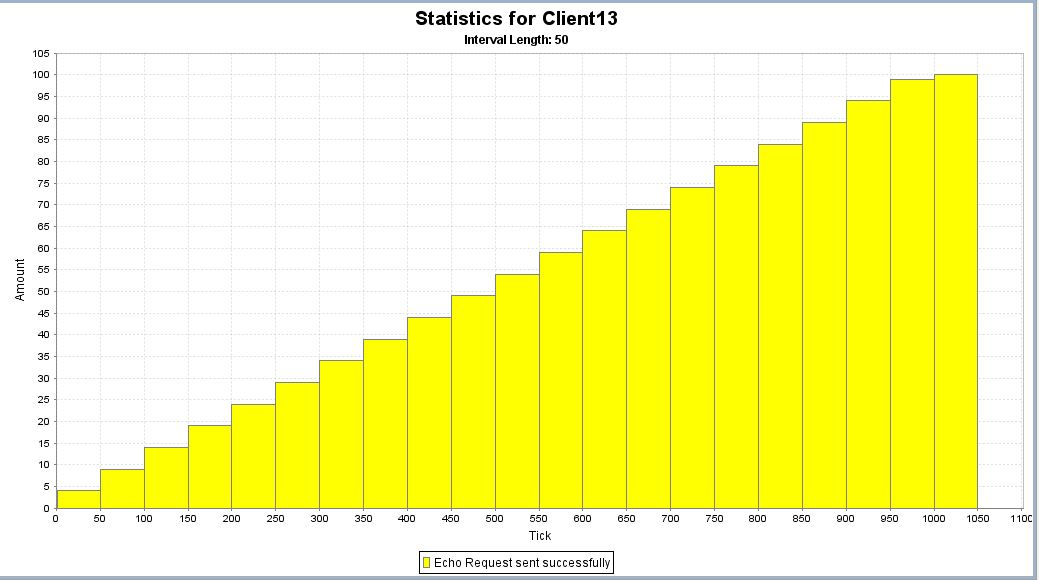
\includegraphics[width=\linewidth]{client.JPG}
	\caption{}
	\label{fig:client54}
\end{figure}












\chapter{Introduction to fog computing}
\label{ch:fog computing}
\section{what is fog computing}
With the rise in smart applications and demand to decrease the latency between the info generation
and processing stage, Cisco coined a brand new term referred to as the fog computing. Fog computing
is the extension of cloud computing towards the network edge to alter cloud-things service time.
It is supported the principle that processing and communication  to be served nearer to the
data sources. Fog computing allows smart applications to perform their processes on network devices which can be routers, gateways or switches instead of causing information to cloud information centers.The principle assures the matter of resource scarcity in IoT as expensive storage, computation and management, and networking may be well offloaded to close fog nodes. This continuously will increase the effectiveness and latency of smart applications. like all services, security mechanisms in IoT can be enforced and deployed at fog layer level, having fog nodes as a proxy, to dump costly storage and computations from IoT devices. Thus, fog nodes give a novel chance for IoT in deploying distributed and collaborative security mechanisms. As compared with cloud computing, fog computing devices can provide less latency for the smart application .
\section{Architecture of fog computing environment}

Fig 1.1 provides a layered architecture of fog computing environment with different devices involved in it. The lowest layer of this architecture contains the data generation devices which can be sensors, RFID tags, cameras, Internet of Things (IoT) devices and actuators. These devices will generate real-time data which should be processed by a smart application to make real-time decisions. Middle layer of the architecture consists of the network devices used to send the data from lower layer devices to the cloud computing infrastructure. This layer can act as a fog layer part or whole computation can be processed so that the application performance is not affected by the latency of the network. Devices in the fog layer are called edge device.
The upper layer is the cloud layer which consists of virtual machines which can be provisioned from any of the cloud service provider. If fog layer does not have free computational resources then it can send the re-quests directly to the cloud infrastructure.
\begin{figure}[h]
	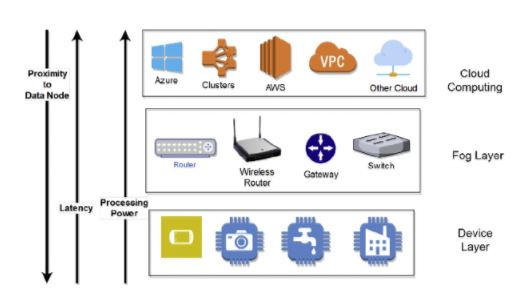
\includegraphics[width=\linewidth]{Capture9.JPG}
	\caption{}
	\label{fig:boat1}
\end{figure}
\section{security in fog computing}
Device security is one in every of the most important challenges for efficient implementation of internet of Things and fog computing atmosphere in current IT house. In fog computing, for any instance of your time same edge device will be utilized by multiple smart applications with totally different set of users that increases the difficulty level of security of edge device. If edge device is hacked, it will get false input and supply false output data, and formulate unnecessary results which  have an effect on the performance of entire application. Hacked device also  want to share information and results with competitive firms or radical teams concerned in unwanted activities. Security protocols that is used currently a days certify every edge device with the application before providing information or computation to perform.

\subsection*{Types of attacks in fog computing}
 If edge device is hacked then scenario becomes even worse as a result of that edge device has certain privileges within the network. So the attack by edge devices on the fog computing setting can be generally characterised into 2 main classes that area unit \textbf{(a) unauthenticated attacks} and\textbf{(b) unauthorized attacks.} If the edge device is unauthenticated and tries to attack the device layer or cloud layer then this attack is named unauthenticated attack or outside attack.But, if the edge device that attacks the fog layer or cloud layer is edge and it's within the given network of application then it's referred to as unauthorized or inside attack.
\subsection*{Attack detection in fog computing}
Though fog computing design can give the required service necessities and distributed resources, robust security mechanisms are required resources to shield IoT devices. As preventive security schemes  with the shortcoming design and implementation flaws, detective mechanisms such as attack detections are inevitable. Attack detections will be either signature primarily based or anomaly
based schemes. The signature primarily based answer matches the incoming traffic against the already identified attack varieties within the info whereas anomaly primarily based theme caters for attack detection as a activity deviation
from traditional traffic. the previous approach has been used widely to its high accuracy of detection and low warning rate, however criticized for its incapability to capture novel attacks. Anomaly detection, on the other hand  detects new attacks although it lacks high accuracy. In these approaches, classical machine learning has been used extensively. With the ever increasing  attackers power and
resources, ancient machine learning algorithms are incapable of police work complicated cyber breaches. The fog nodes are answerable for training models and hosting attack detection systems at the edge of the distributed fog network.




 











\chapter{Introduction to Deep learning}
\label{ch:deep learning}

Deep learning in security learns real face (attack or legitimate) of cyber information on even little
variations or changes, indicating the resiliency of deep learning to little changes in network information by
creating high level invariant representations of the training information. Machine learning refers to systems
that  measure ready to mechanically improve with expertise. historically, in spite of what number times you
use system to perform an equivalent actual task, the system won’t get any smarter. Whenever we launch our
browser and visit an equivalent actual website? a conventional browser won’t ”learn” that it ought to most likely
just bring you there by itself once 1ist launched. With ML, package will gain the power to be told from
previous observations to form inferences regarding  future behavior, moreover as guess what you would like to
do in new situations.  However to understand how ML works we tend to 1ist have to be compelled to understand the fuel that creates ML (data)
possible: information(data). think about associate email spam detection algorithmic rule. Original spam filters would merely blacklist
certain addresses and permit alternative mail through. ML increased this significantly by scrutiny verified
spam emails with verified legitimate email and seeing that ”features” were gift additional oft in
one or the opposite. as an example, designedly misspelled words,the presence of hyperlinks
to best-known malicious websites, and virus-link attachments  measure doubtless options indicative of spam rather
than legitimate email. (More discussion on ”features” below.) This method of mechanically inferring a
label (i.e., ”spam” vs ”legitimate”) is named classification, and is one amongst the foremost applications of ML
techniques. it's price mentioning that one alternative quite common technique is prognostication, the use of
historical information to predict future behavior.

\section{security using Deep learning}
DL has many variants whose quality depends on the character of the appliance . Autoencoder
and its families are the foremost applied  models, and have resulted in promising leads to unattended
learning. Autoencoder map input options a similar range of output options, minimizing
reconstruction errors.In different word, given a collection of untagged training knowledge x(1), x(2), x(3), , stacked
autoencoder maps to output options to be up to the input options (i.e., y(i) = x(i)). Technically, autoencoding
is a compress-decompress technique of pattern extraction from knowledge. The drawbacks of classical
machine learning in attack detection and lack of automatic feature engineering, low detection rate, and incapability of detection tiny mutants of existing attacks and zero-day attacks. These limitations will
be improved by adopting DL. By making high-level representations of options, DL discovers advanced
functions that map input to output without manual intervention by consultants. DL additionally exploits the advantages
of automatic hierarchic feature learning from data. Attack detection may gain advantage from a
pre-training theme of stacked autoencoders for automatic feature learning. a way to use stacked
autoencoder is to train a model with a mixture of normal/attack sample of the untagged network so the
model identifies patterns of attack and traditional knowledge by a self-learning theme. The detected patterns 
mapped to labelled check knowledge as attack and traditional.

and normal. 

\chapter{Attack Detection using deep learning}
\label{ch:Attack deep learning}
\section{Our Work}
(1) To design and implement deep learning based attack detection mechanism.

(2) This work has used self taught deep learning scheme in which unsupervised feature learning has been employed on training data.

(3) The learnt features were applied to the labeled test dataset for classification into attack and normal.
\section{Dataset description}
We used NSL-KDD intrusion dataset which is available in csv format for
model validation and evaluations.
The original dataset consists of 125,973 records of train and 22,544 records of test, each with 41 features such as duration,protocol, service, flag, source bytes, destination bytes, etc.

\begin{figure}[h]
	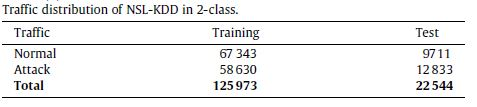
\includegraphics[width=\linewidth]{Capture17.JPG}
	\caption{}
	\label{fig:boat1}
\end{figure}
\newpage
\begin{figure}[t]
	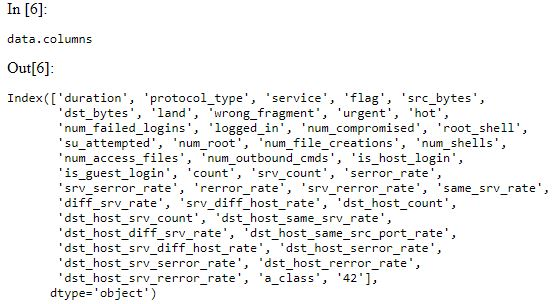
\includegraphics[width=\linewidth]{Capture10.JPG}
	\caption{columns of dataset}
	\label{}
\end{figure}
\begin{figure}[h]
	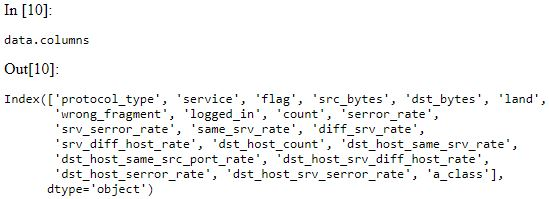
\includegraphics[width=\linewidth]{Capture11.JPG}
	\caption{columns of dataset after droping some columns}
	\label{}
\end{figure}

\section{Our Approach}
\textbf{ToolS/Framework Used -}  Anaconda, Spider IDE, Keras, Sklearn .

\textbf{Anaconda} is complete development environment with over 300 Python packages.Conda is a powerful package manager and environment manager that you use with command line commands at the Anaconda Prompt.

\textbf{Keras} is a high-level neural networks API, written in Python and capable of running on top of TensorFlow, CNTK, or Theano.

The core data structure of Keras is a model, a way to organize layers. The simplest type of model is the Sequential model, a linear stack of layers. For more complex architectures, you should use the Keras functional API, which allows to build arbitrary graphs of layers.

Before training the network, categorical features have been encoded into discrete features using 1-to-n encoding technique.
\newline
\textbf{Labelencoder()} is a utility function to help normalize labels such that they contain only values between 0 and n\_classes-1.

\textbf{fit\_transform()} joins two steps and first step is  initial fitting of parameters on the training set,in second step it returns a transformed set. Internally, it just calls first fit() and then transform()on the same data.

\textbf{MinMaxScaler} Transforms features by scaling each feature to a given range.
This translates each feature individually such that it is in the given range on the training set, i.e. between zero and one.

\textbf{k-Fold Cross Validation} 
\newline
The main standard for machine learning model evaluation is k-fold cross validation.
It provides a estimate of the performance of a model on unseen data. It does this by splitting the training dataset into k subsets and takes turns training models on all subsets except one which is held out, and evaluating model performance on the held out validation dataset. The process is repeated until all subsets are given an opportunity to be the held out validation set. The performance measure is then averaged across all models that are created.
Cross validation is often not used for evaluating deep learning models because of the greater computational expense. For example k-fold cross validation is often used with 5 or 10 folds. As such, 5 or 10 models must be constructed and evaluated, greatly adding to the evaluation time of a model.
Nevertheless, it when the problem is small enough or if you have sufficient compute resources, k-fold cross validation can give you a less biased estimate of the performance of your model.
In our approach we used the handy StratifiedKFold class from the sk-learn Python machine learning library to split up the training dataset into 10 folds. The folds are stratified, meaning that the algorithm attempts to balance the number of instances of each class in each fold.

\newpage
\begin{figure}[h]
	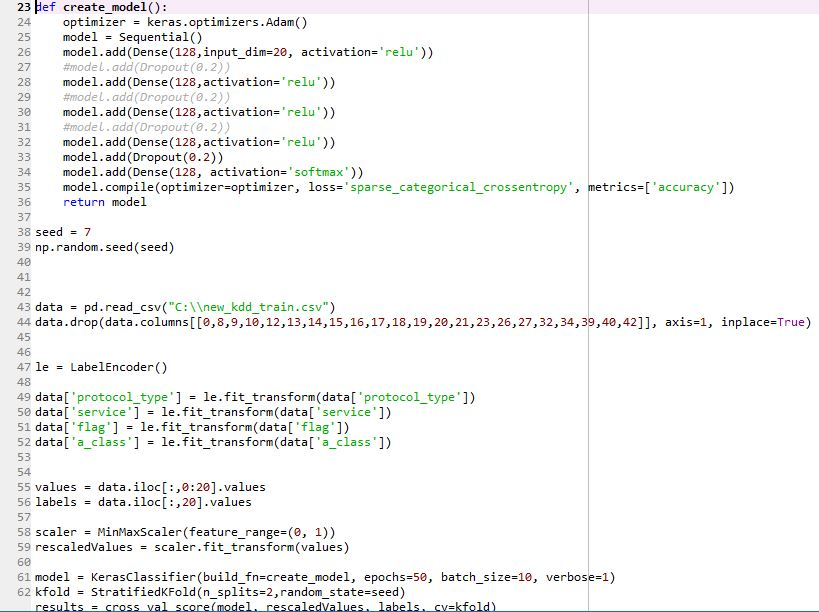
\includegraphics[width=\linewidth]{Capture19.JPG}
	\caption{}
	\label{fig:boat1}
\end{figure}

\newpage
\section{Accuracy of our model :}
\begin{figure}[h]
	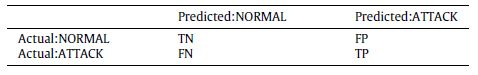
\includegraphics[width=\linewidth]{Capture14.JPG}
	\caption{}
	\label{fig:boat1}
\end{figure}
\begin{figure}[h]
	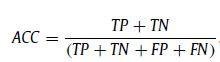
\includegraphics[width=\linewidth]{Capture15.JPG}
	\caption{Accuracy Formula}
	\label{fig:boat1}
\end{figure}
\begin{figure}[h]
	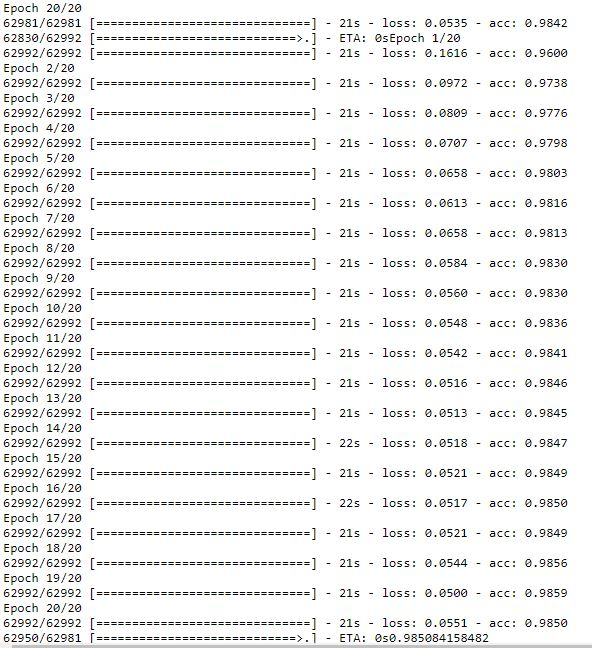
\includegraphics[width=\linewidth]{Capture12.JPG}
	\caption{Accuracy}
	\label{fig:boat1}
\end{figure}





\chapter{Conclusions and Future Work}
\label{ch:conclude}
\section{conclusion}
This work mainly focus on attacks possible in cloud computing and what are mitigations to these attacks.
This work also proposes simulation model suitable for the detection of DDoS attacks. The obtained simulation results demonstrates the effective dangerousness of the amplification attacks that permit to a single host to generate an huge volume of traffic by exploiting infected hosts (botnet) and vulnerable servers. The developed model constitutes a valuable tool for easing the study of the effects of such types of attacks.

\section{Scope of further work}
(1) DDOS attacks are launched using well coordinated and highly organized attack network. the ISPs are also required to work in tandem for designing technical and economic models to achieve cooperation, in order to fight against the menace of Ddos attacks collaboratively.

(2) we have to develop a model to prevent DDOS attack using Nessi2. 




%--------------------------------------------------------

%--------------------------------------------------------
%%% Optional appendix
%\appendix
%\chapter{}
%\label{}

%--------------------------------------------------------
% Recommended 'Related Publication'
%--------------------------------------------------------

\bibliographystyle{latex8}
\bibliography{sampleBib} 

\end{document}
